\chapter{Paleointensity}



%\HCode{<a name="IE-R"></a>}


 A complete understanding of the geomagnetic field requires not only a description of the direction of field lines over the surface of the Earth, but information about its strength as well.  While directional information is relatively straight-forward to obtain, intensity variations are much more difficult and are the subject of  this chapter.


 In principle, it is possible to determine the
intensity of ancient magnetic fields $\B_{anc}$ because  common mechanisms
by which rocks become magnetized (e.g., thermal, chemical and detrital remanent
magnetizations) 
are frequently  approximately linearly related to the 
ambient field for
low fields such as the Earth's (Chapter 7 and Figure~\ref{fig:pintprinc}), i.e.,
 
 $$
 M_{NRM}   = \nu_{anc} B_{anc},
 $$
 \noindent and
 $$
 M_{lab}  =  \nu_{lab} B_{lab}.
 $$
 
\noindent  where $\nu_{lab}$ and $\nu_{anc}$ are constants of proportionality. If the two constants  are the same, we can divide the two  equations and rearrange them to get:

\begin{equation}
{B_{anc} }=  {M_{NRM} \over {M_{lab}}}{B_{lab} }.
\label{eq:banc}
\end{equation}
 
 \noindent  If the laboratory remanence has the same proportionality constant with respect to the applied field  as the ancient one,  the remanences  were linearly related to the applied field, and the NRM comprises a single component, all one need do  to get the ancient field is  measure the NRM,
and determine $\nu$ by giving the rock a laboratory remanence in a known field ($B_{lab}$).  Multiplying the ratio of the two remanences by the  lab field would give the ancient magnetic field.  
 
 \begin{figure}[htb]
%\epsfxsize 8cm
%\centering \epsffile{EPSfiles/pintprinc.eps}
\centering  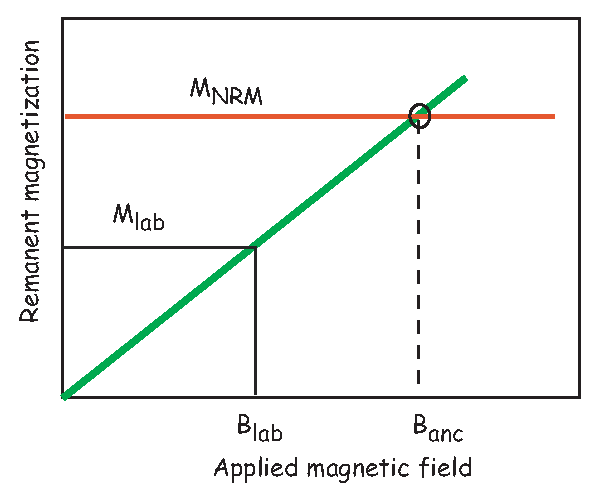
\includegraphics[width= 8 cm]{EPSfiles/pintprinc.eps}
\caption{Principles of  paleointensity estimation.  The remanent magnetization is assumed linear with the magnetic field. If the slope $\nu$ can be determined through laboratory proxy measurements ($M_{lab}/B_{lab}$), then the  NRM of a given specimen, $M_{NRM},$ can be mapped to an estimate of the ancient magnetic field $B_{anc}$.}
\label{fig:pintprinc}
\end{figure}


The theory just outlined is quite simple, yet, in practice, recovering paleointensity is not simple; there are many causes for concern:

\begin{enumerate}
\item  The proportionality ``constant'' $\nu$ may not be constant at all because the NRM acquisition may not be even approximately linear with the applied field (see Figure~\ref{fig:trm}).   
\item  The specimen may have altered its capacity to acquire remanence (changing $\nu_{lab}$) either through weathering or other chemical alteration or during the acquisition of the laboratory remanence.
\item If the original NRM is carried by multi-domain or even ``PSD'' grains in what we called pseudo-multi-domain grain size,  the exact conditions of NRM acquisition will be difficult to reproduce because unblocking may occur at a different temperature than blocking. 
\item  If the specimen is anisotropic in its remanence acquisition and the laboratory field is not parallel to the ancient field direction, the two proportionality constants can be quite different.   In fact, $\nu$ is a tensor and the scalar approximation at times fails badly.
\item If the NRM  was acquired by a mechanism difficult to reproduce in the laboratory, the normalization will be more difficult or even impossible.   For example  CRMs and  DRMs,   are very difficult to reproduce exactly.  Moreover if a TRM was acquired over a  timescale inaccessible to laboratory experiment (cooling of a pluton), the relationship between $\nu_{anc}$ and $\nu_{lab}$ may be different by as much as a factor of two.  
\item  If the natural remanence comprises  multiple  components, for example, an original remanence plus a viscous or isothermal one, it may be difficult to isolate the primary remanence and normalize it properly.   
\end{enumerate}


    In this chapter we will discuss the assumptions behind paleointensity estimates and outline various experimental and statistical  methods involved in  getting paleointensity  data.    We will start by considering thermal remanences and  then address depositional ones.    To our knowledge, no one has deliberately attempted paleointensity estimation  using other remanence types such as chemical or viscous remanences although both are theoretically possible.

%\HCode{<a name="LT-TI"></a>}
\section{Paleointensity with TRMs}


  The  theoretical basis for how ancient magnetic fields might be preserved was laid out by   L.  N\'eel  (see Chapter 7).  We expect thermal remanences of quasi-equant single domain particles  to be linearly related to the applied field for low fields like the Earth's (although elongate particles may not behave linearly even in low fields).    Larger particles of magnetite   have more complicated remanent states (flower, vortex, multi-domain)  and  TRM acquisition curves is more difficult to predict from theory.  However, empirical studies have shown that TRM acquisition is significantly  non-linear even at rather low field strengths and that the departure from non-linearity is grain size dependent; the larger the particle, the lower the field at which non-linearity becomes an issue  (e.g.,
  \index{Dunlop, D.J.}   
  \index{Argyle, K.S.}
Dunlop and Argyle,  1997).   \nocite{dunlop97b}   Nonetheless, the largest intensities on the Earth today ($\sim$65 $\mu$T) are within the linear region  for small equant particles and one could  reach several hundred microtesla before having to worry about non-linearity.    Therefore the linearity assumption  appears to be reasonably well founded for ideal assemblages.  Indeed, the linearity assumption is so deeply embedded in paleomagnetic practice that it is almost never tested! However,  it has recently become evident that naturally occurring assemblages of single domain magnetite can have significantly non-linear TRM acquisition behavior 
  \index{Selkin, P.}
  %\customlink{non-linear_TRM}
  (Selkin et al., 2007), \nocite{selkin07} even for fields as low as the  Earth's (see Figure~\ref{fig:trm}).  Because the exact form of the TRM acquisition depends critically on the magnetic assemblage,  it would be wisest to include a TRM acquisition experiment in any paleointensity experiment.  
  

There are several ways of checking the ability of the specimen to acquire TRM in paleointensity experiments.  In Section~\ref{sect:KTT}  we will discuss the
\index{paleointensity method!step-wise heating}
step-wise heating  and 
\index{paleointensity method!Shaw}
{\it Shaw} methods.   Other approaches attempt to prevent the alteration from occurring, for example by using microwaves to heat just the magnetic phases, leaving the rest of the specimen cool, or by minimizing the number of heating steps.  Some methods attempt to normalize the remanence with IRM and avoid heating altogether.  We will briefly describe each of these in turn, beginning with the step-wise heating family of experiments.   Regardless of method chosen,  it is essential that as many of the assumptions in the experiment be tested as possible.  Experiments that skirt the issues involved simply give us data whose reliability can not be verified and, given all the things that can go wrong, such data are essentially useless.   



\subsection{Stepwise heating  family of  experiments}
\label{sect:KTT}

A goal in paleointensity experiments since the earliest days has been the detection of changes in the proportionality constant caused by alteration of the magnetic phases in the rock during heating (e.g., Thellier and Thellier, 1959). \nocite{thellier59}   
The basic idea is to heat specimens up in stages, progressively replacing the natural remanence with  partial thermal remanences.    The step-wise heating
\index{paleointensity method!double-heating}
  approach is particularly powerful when lower temperature    steps are repeated, to verify directly  that the ability to acquire a  thermal remenance has not changed.   
  
   The step-wise heating approach relies on the assumption that partial thermal remanences (pTRMs) acquired by cooling between any two temperature steps (e.g., 500$^{\circ}$ and 400$^{\circ}$C in Figure~\ref{fig:ptrm}  of Chapter 7) are independent of those acquired between any other two temperature steps.  This assumption is called the 
   \index{Law of!independence}
{\it Law of Independence} of  pTRMs.  The approach also assumes that the total TRM is the sum of all the independent pTRMs (see Figure~\ref{fig:ptrm}), an assumption called the 
\index{Law of!additivity}
{\it Law of  Additivity}  
   
\begin{figure}[h!tb]
%\epsfxsize 7cm
%\centering \epsffile{EPSfiles/koenigsberger.eps}
\centering  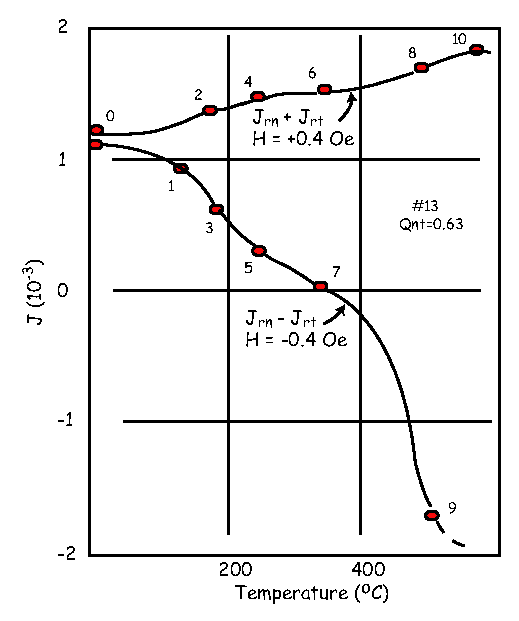
\includegraphics[width= 7 cm]{EPSfiles/koenigsberger.eps}
\caption{Example of thermal normalization experiment of K\"onigsberger (1938).  A specimen is heated to given temperature and cooled in a field of +0.4 Oe (40 $\mu$T) (e.g., step labeled \#4).  Then the specimen is heated to same temperature and cooled in field of -0.4 Oe (e.g., step \#5).  The two curves can be decomposed to give $M_{nrm}$ and $M_{lab}$, the ratio of which was termed $Q_{nt}$ by K\"onigsberger.  Note that $J_{rn}$ and $J_{rt}$ are $M_{NRM}$ and $M_{pTRM}$ respectively here. [Figure redrawn from K\"onigsberger (1938) by Tauxe and Yamazaki, 2007.]}
\label{fig:koenigsberger}
\end{figure} \nocite{koenigsberger38}
  
There are many possible  ways  to progressively replace the NRM with a pTRM in the laboratory.  In the original step-wise heating method (e.g., K\"onigsberger, 1938)  the specimen is heated twice and cooled in the laboratory field; we will call this  the ``infield-infield'' or ``II'' method.    The first step is  to heat the specimen to some temperature ($T_1$) and cool it  in the laboratory field $B_{lab}$.  Measurement of  the combined remanence (what is left of the natural remanence plus the new laboratory pTRM) yields:

$$
 \M_{1} = \M_{NRM} + \M_{ pTRM}. 
$$
\noindent  Then the specimen  is heated a second time and cooled upside down (in field $-B_{lab}$).  The second remanence is therefore:

$$
 \M_{2} = \M_{NRM} -\M_{ pTRM}. 
$$
\noindent Simple vector subtraction allows the determination of the NRM remaining at each temperature step and the pTRM gained.  An example of data from one of K\"onigsberger's experiments is shown in Figure~\ref{fig:koenigsberger}. The two curves are obtained through successive temperature steps,  $\M_1(T)$ and $\M_2(T)$  (called $J_{rn}+J_{rt}$ and $J_{rn}-J_{rt}$ respectively by 
\index{K\"onigsberger, J.G.}
\nocite{koenigsberger38}
K\"onigsberger, 1938).  For each step, $\M_{NRM}$ and $\M_{pTRM}$ could be estimated and the ratio gave an estimate of $\B_{anc}$ (called $Q_{nt}$ by K\"onigsberger).   The II method implicitly assumes that a magnetization acquired by cooling from a given temperature is entirely replaced by re-heating to the same temperature (i.e., $T_b=T_{ub}$), an assumption known as the 
\index{Law of!reciprocity}
{\it Law of Reciprocity}.  

As magnetic shielding improved,  modified protocols were developed.  
In the most popular paleointensity  technique (usually attributed to 
\index{Coe, R.S.}
Coe,  1967), \nocite{coe67} we substitute cooling in zero field for the first heating step.  This  allows  the direct measurement of the NRM remaining at each step.   The two equations now are:

$$
 \M_1 = \M_{NRM},   
$$
\noindent and
$$
 \M_2 = \M_{NRM} + \M_{ pTRM}. 
$$

\noindent  The laboratory  $\M_{ pTRM}$ in this ``zero-field/in-field'' (or ZI) method is calculated by  vector subtraction.  Alternatively, the first heating and cooling can be done in the laboratory field and the second in zero field
\index{Aitken, M.J.}
 (Aitken et al., 1988),  \nocite{aitken88} here called the ``in-field/zero-field'' or (IZ) method.  As the NRM decays, the pTRM grows (Figure~\ref{fig:thellier}a).  Such data are  nowadays plotted against each other in what is usually called an 
\index{diagrams!Arai}
{\it Arai diagram} 
\index{Nagata, T.}
 (Nagata et al.,  1963) \nocite{nagata63} as in Figure~\ref{fig:thellier}b. 


\begin{figure}[htb]
%\epsfxsize 14cm
%\centering \epsffile{EPSfiles/TT.eps}
\centering  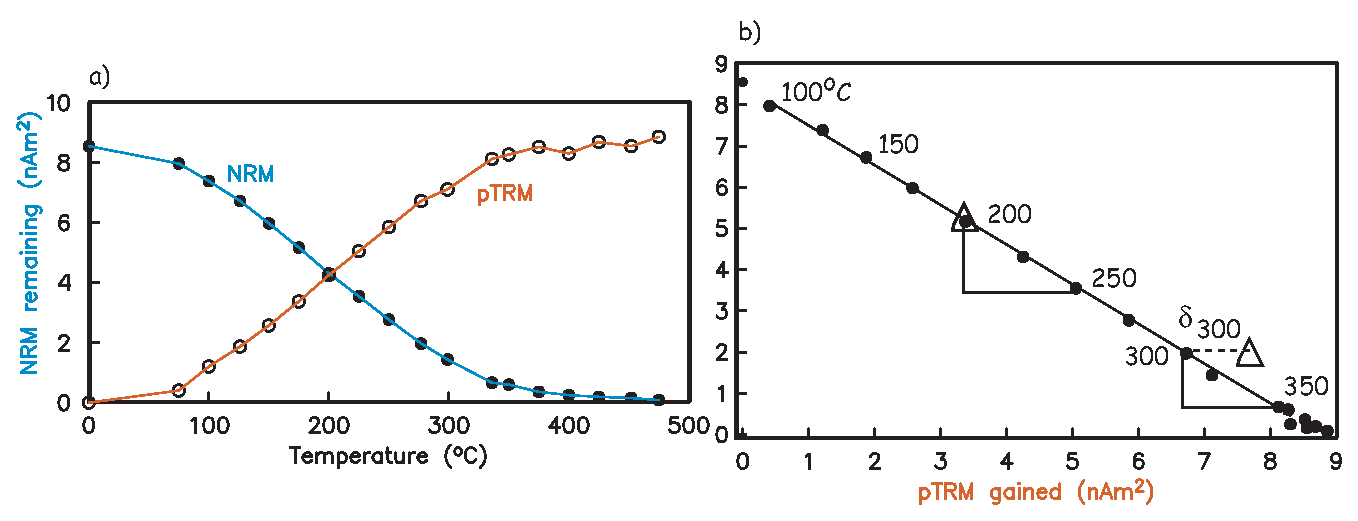
\includegraphics[width= 14 cm]{EPSfiles/TT.eps}
\caption{Illustration of step-wise heating method for determining absolute paleointensity.  a) Thermal demagnetization of NRM shown as filled circles and the laboratory acquired pTRM shown as open symbols.  b) Plot of NRM component remaining versus pTRM gained at each temperature step.  Triangles are the second in-field heating step (pTRM check step) at  a given temperature.  The difference, e.g., $\delta_{300}$, is an indication of possible alteration during the heating experiment. }
\label{fig:thellier}
\end{figure}


In all three of these experimental designs  (II, ZI and IZ),  lower temperature in field cooling steps can be repeated to determine whether the remanence carrying capacity of the specimen has changed (e.g., Thellier and Thellier, 1959). \nocite{thellier59}    These steps are called  
\index{pTRM!checks}
{\it pTRM checks}  (triangles in Figure~\ref{fig:thellier}b).   Differences between the first and second  $M_{ pTRM}$s at a given temperature indicate a change in capacity for acquiring thermal remanences (e.g., $\delta_{300}$ in Figure~\ref{fig:thellier}b)  and are grounds for suspicion or rejection of the data after the onset of such a change.  
 [Some experiments repeat lower temperature zero field steps but these are not strictly pTRM checks (although they are called that) because they really test whether the NRM remaining at that temperature has been contaminated by unremoved pTRM tails or CRM.]
%Some have proposed that paleointensity data can be ``fixed'' even if they pTRM checks show significant alteration (e.g., Valet et al., 1996).  The argument is that if pTRM checks can be brought back into accordance with the original pTRM measurements using a correction factor, then if that same correction factor is applied to all subsequent pTRM measurements, the effect of the alteration has been accounted for and the data can be considered ``reliable''.  We consider this correction to carry considerable  risk and ``corrected'' data should be clearly marked as such.      


Despite its huge popularity and widespread use, the  approach of progressively replacing the natural remanence with a thermal remanence has several drawbacks.  Alteration of the ability to acquire a pTRM is not the only cause for failure of the assumption of equality of $\nu_{lab}$ and $\nu_{anc}$.  Single domain theory and the 
\index{Law of!reciprocity}
Law of Reciprocity required by all step-wise heating methods assumes that the remanence acquired by cooling through a given  temperature interval is entirely removed by re-heating to the same temperature and cooling in zero field.   Yet both  experiment 
\index{Bol'shakov, A.S.}
\index{Shcherbakova, V.V.}
(Bol'shakov and Shcherbakova, 1979) \nocite{bolshakov79} and theory 
\index{g, D.J.}
\index{Xu, S.}
(e.g., Dunlop and Xu, 1994) \nocite{dunlop94} suggest that the essential assumption of equivalence of blocking and unblocking temperatures may break down for larger particles.   

\begin{figure}[htb]
%\epsfxsize 14cm
%\centering \epsffile{EPSfiles/dunlop01.eps}
\centering  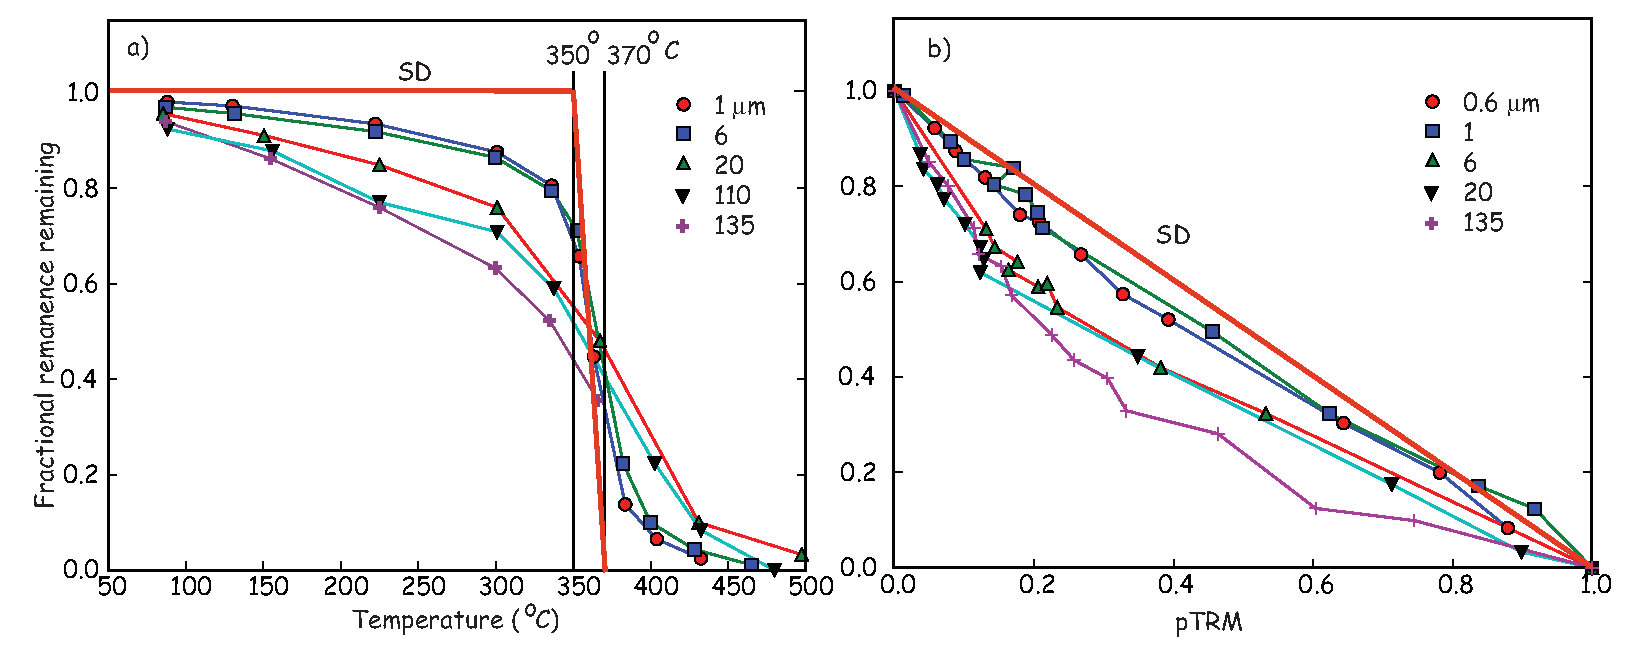
\includegraphics[width= 14 cm]{EPSfiles/dunlop01.eps}
\caption{ a) Stepwise thermal demagnetization of pTRMs imparted  by applying a  small DC field during cooling from 370 to 350$^{\circ}$C in magnetite specimens of known grain size.  
Between  50 and 90\% of the remanence unblocks at temperatures below (a low temperature pTRM tail) or above (a high temperature pTRM tail)  the pTRM blocking
temperature range.  The failure of reciprocity  is most extreme for the largest grain sizes.     b) Step-wise heating   paleointensity experiments on specimens with a  laboratory TRM.  Heavy red line is theoretical SD behavior.   All specimens give results that sag below the ideal SD line, an expression of the pTRM tails exhibited by some of the same specimens in a).   [Data of Dunlop and \"Ozdemir, 2001.] }
\label{fig:dunlop01}
\end{figure} \nocite{dunlop01}


\index{Dunlop, D.J.}
\index{\"Ozdemir, \"O.}
Dunlop and \"Ozdemir (2001)   illustrated the failure of the  reciprocity assumption with a suite of specimens whose grains sizes were well known.  First, they  imparted a pTRM over a narrow temperature interval of 370--350$^{\circ}$C . They then subjected the specimens to step-wise thermal demagnetization, monitoring the remanence remaining after each treatment step (see Figure~\ref{fig:dunlop01}a.)    The heavy red line labelled ``SD'' is the prediction from the 
\index{Law of!reciprocity}
law of reciprocity.  This assumption is not met by any of the specimens (the smallest of which was 0.6 $\mu$m,  much larger than SD) and the larger the grain size, the larger the deviation from theory.   The portion of pTRM lost by heating to temperatures below the blocking temperature is a low-temperature 
\index{pTRM!tails}
{\it pTRM tail}  and that above is a high temperature pTRM tail.     These tails have a profound affect on the outcome of double heating  experiments as shown in Figure~\ref{fig:dunlop01}b.    The data sag below the ideal line, becoming markedly curved for  grains larger than about a micron.   


What causes failure of reciprocity?   
If the particle is large enough to have domain walls in its remanent state,   the behavior is  not easily understood by theory.  At just below its Curie Temperature  the particle would be at saturation.    As the particle cools,  domain walls will begin to form at some temperature.  After cooling all the way to room temperature, the  remanent state, it  will have some net moment because the domain walls will distribute themselves such that there is incomplete cancellation leaving a small net remanence proportional to the applied field for moderate field strengths.  As the temperature ramps up again, the walls  ``walk around'' within the particle, perhaps beginning below the blocking temperature as they seek to minimize the magnetostatic energy.  If the particle is cooled back to room temperature, there could be  a net loss of magnetization, giving rise to low temperature tails.  The walls may  not actually be destroyed until the  temperature is very near the Curie Temperature and some fraction of the pTRM could persist,  giving rise to high temperature tails.  


A failure of reciprocity means that $\nu_{lab} \neq \nu_{anc}$ and the key assumptions of the step-wise heating type methods are not met.  The  Arai plots  may be curved as in Figure~\ref{fig:dunlop01}b.   If any portion of the NRM/TRM data are used  instead of the entire temperature spectrum, the result could be biased.  For example,  the lower temperature portion might be selected on the grounds that the higher temperature portion is affected by alteration. Or, the higher temperature portion might be selected on the grounds that the lower temperature portion is affected by viscous remanence.  Both of these interpretations are  wrong.   

\begin{figure}[h!tb]
%\epsfxsize 14.5cm
%\centering \epsffile{EPSfiles/method.eps}
\centering  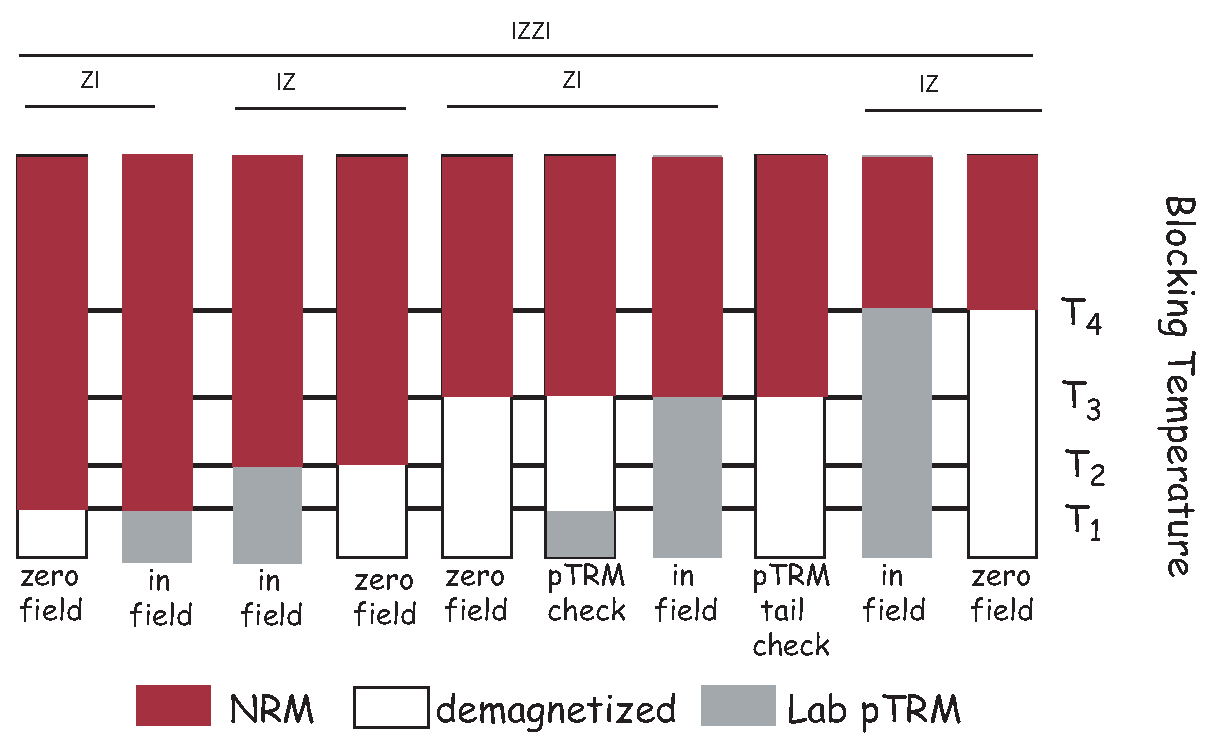
\includegraphics[width= 14.5 cm]{EPSfiles/method.eps}
\caption{Schematic diagram of the  IZZI experimental protocol.  [Figure from Ben-Yosef et al., 2008.]    }
\label{fig:method}
\end{figure}
  \nocite{benyosef08}


In order to detect inequality of blocking and unblocking and the effect of  ``pTRM tails'',  several embellishments to the step-wise heating experiments have been proposed and more are on the way.  One modification is to alternate between the IZ and ZI procedures (the so-called 
\index{paleointensity method!IZZI}
{\it IZZI method}  of, e.g.,  
\index{Tauxe, L.}
\index{Staudigel, H.}
Tauxe and Staudigel (2004; see also  \nocite{tauxe04} 
\index{Ben-Yosef, E.}
Ben-Yosef et al., 2008).   \nocite{benyosef08}  The protocol shown in     Figure~\ref{fig:method} not only alternates ZI and IZ steps, but embeds a pTRM check step within each ZI step.  There is also a third zero field step inserted between the ZI and IZ steps, labelled
\index{pTRM!tail check}
{\it pTRM-tail check}.
This step was first described by
\index{Dunlop, D.J.}
\index{\"Ozdemir, \"O.}
\nocite{dunlop97} Dunlop and \"Ozdemir (1997) but is usually attributed to
\index{Riisager, P.}
\index{Riisager, J.}
Riisager and Riisager (2001). \nocite{riisager01}  It was designed to assess whether the  partial thermal remanence gained in the laboratory at a given temperature is completely removed by re-heating to the same temperature.  The difference between the two zero-field steps is attributed to  a ``pTRM tail''.    In the original application, the absolute value of the difference was plotted on the vertical axis 
\index{Dunlop, D.J.}
\index{\"Ozdemir, \"O.}
(Dunlop and \"Ozdemir, 1997; see also Riisager and Riisager, 2001) 
and was interpreted to be   a consequence of an inequality of the unblocking temperature $T_{ub}$ and the original blocking temperature $T_b$ in violation of the 
\index{Law of!reciprocity}
law of reciprocity.  The IZZI method is extremely sensitive to the presence of  pTRM tails which make the 
\index{diagrams!Arai}
\index{diagrams!Zijderveld}
and/or Zijderveld  diagrams 	``zig-zag'' as in the  example of a complete IZZI experiment shown in Figure~\ref{fig:zigzag}.    The zig-zag behavior was explained by 
\index{Yu, Y.}
Yu et al. (2004) as the effect of  pTRM tails.  \nocite{yu04}
 
  In Figure~\ref{fig:zigzag}, we plot the  pTRM tail checks from a typical experiment as blue squares along the X axis;  note that these are not absolute values, but are the magnitudes of the differences in zero field steps separated by an in-field step at the same temperature.  We plot them this way because what is being measured is a difference in the NRM remaining, not the pTRM.  It is perhaps surprising that most pTRM tails appear to be negative -- not positive, suggesting the dominance of  low temperature tails, as opposed to  high temperature tails. Note also that the IZ steps are typically farther from the ideal line than are the ZI steps.  In any case, significant zig-zagging should raise warning flags about the reliability of data acquired by such non-ideal specimens.  

 

\begin{figure}[h!tb]
%\epsfxsize 14cm
%\centering \epsffile{EPSfiles/zigzag.eps}
\centering  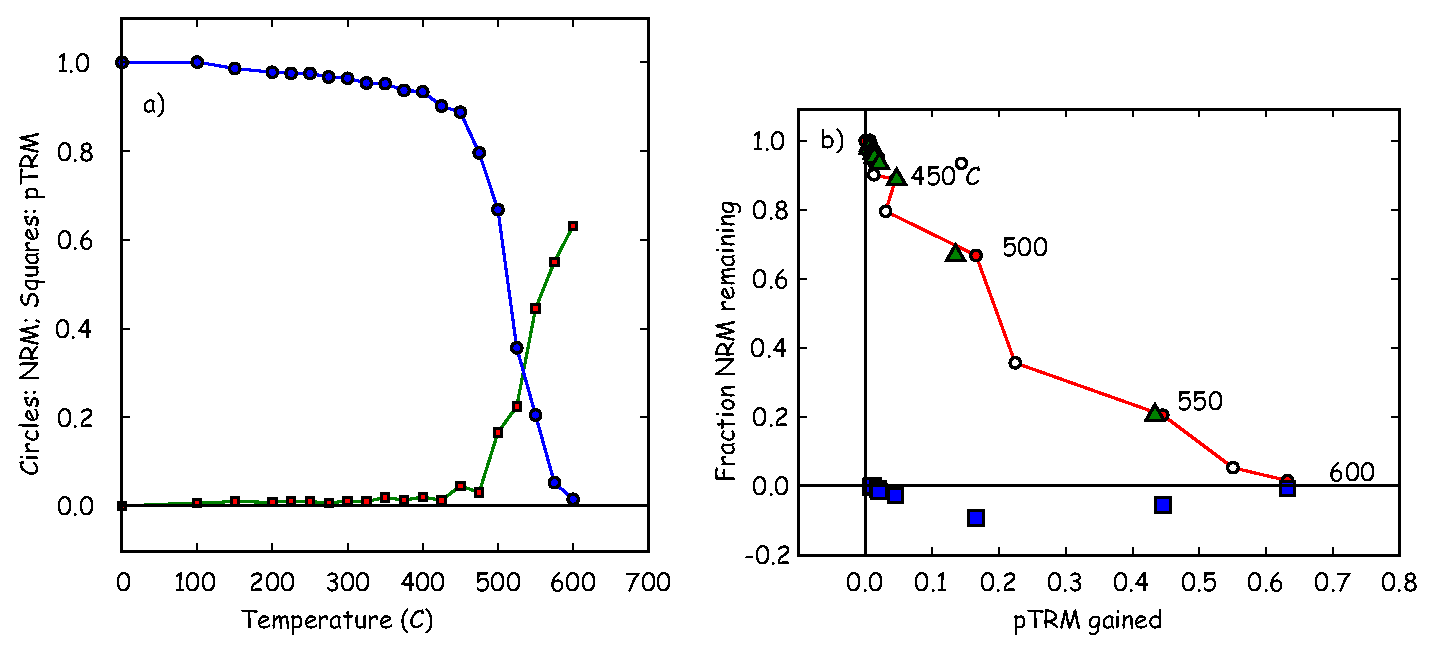
\includegraphics[width= 14 cm]{EPSfiles/zigzag.eps}
\caption{Example of results from an IZZI paleointensity experiment.  a) NRM remaining after demagnetization in zero field (blue circles) and pTRM gained after heating and cooling  in the laboratory field (red squares).  Both remanences were normalized by the initial NRM.   b) Arai plot of data in  a).   Open (closed) symbols are the IZ (ZI) steps.  Triangles are pTRM check steps and blue squares are the pTRM tail check steps.    The zig-zag behavior is characteristic of the effect of pTRM tails. }
\label{fig:zigzag}
\end{figure}



There are several other violations of the fundamental assumptions that require additional tests 
 and/or corrections in the paleointensity experiment besides alteration or failure of  reciprocity.   For example, if the specimen is anisotropic with respect to the acquisition of thermal remanence (e.g., 
 \index{Aitken, M.J.}
Aitken et al., 1981), \nocite{aitken81} the  TRM can be strongly biased (Figure~\ref{fig:trm-anis}).  If this is the case, the TRM can be corrected by determining the TRM  (or the ARM proxy) anisotropy tensor and matrix multiplication to recover the original magnetic vector (see Section~\ref{sect:aarm} in Chapter 13 and 
 \index{Selkin, P.}
 Selkin et al., (2000), for a more complete discussion.) \nocite{selkin00b}   One quick way of detecting if anisotropy might be a problem is to compare the direction of the pTRM acquired in the laboratory with the laboratory field direction, a parameter called $\gamma$ in Appendix~\ref{app:pint} .  If this angle exceeds  $\sim 5 ^{\circ}$,  the anisotropy tensor should be determined.   This will not  work if the lab field is applied near the principal direction where only a change in magnitude is expected, but does work if the laboratory field is applied at an angle to the principal direction. 
 
\begin{figure}[h!tb]
%\epsfxsize 9cm
%\centering \epsffile{EPSfiles/trm-anis.eps}
\centering  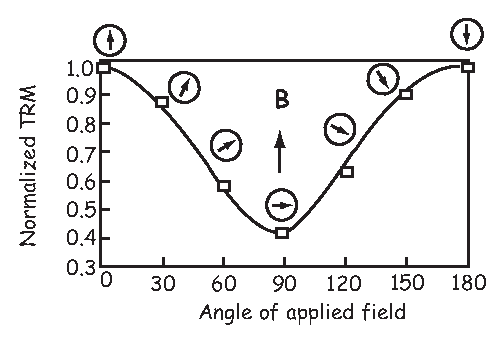
\includegraphics[width= 9 cm]{EPSfiles/trm-anis.eps}
\caption{Data from an experiment with an anisotropic specimen given a total TRM in different orientations with respect to the laboratory field.  The relative TRM magnitudes are plotted as squares and a best fit model intensity based on the TRM anisotropy tensor is shown as the solid line.  [Redrawn from Selkin et al., 2000.]}
\label{fig:trm-anis}
\end{figure}


 
 Differences in laboratory and ancient cooling rate are also important. The approach to equilibrium is a function of time. Slower cooling results in a larger TRM, hence differences in 
 \index{cooling rate}
 cooling rate between the original remanence acquisition and that acquired in the laboratory will
 lead to erroneous results (e.g., 
 \index{Halgedahl, S.}
 Halgedahl et al., 1980).   \nocite{halgedahl80}   Compensating for differences in cooling rate is relatively straight-forward if the  original cooling rate is  known  or can be approximated and the specimens behave according to single domain theory (see Figure~\ref{fig:coolingrate}).  Alternatively, one could take an empirical approach in which the rock is allowed to acquire a pTRM under varying cooling rates (e.g., 
 \index{Genevey, A.}
 \index{Gallet, Y.}
 Genevey and Gallet, 2003),       \nocite{genevey03}
  an approach useful for cooling rates of up to a day or two.  
 
\begin{figure}[htb]
%\epsfxsize 10cm
%\centering \epsffile{EPSfiles/coolingrate.eps}
\centering  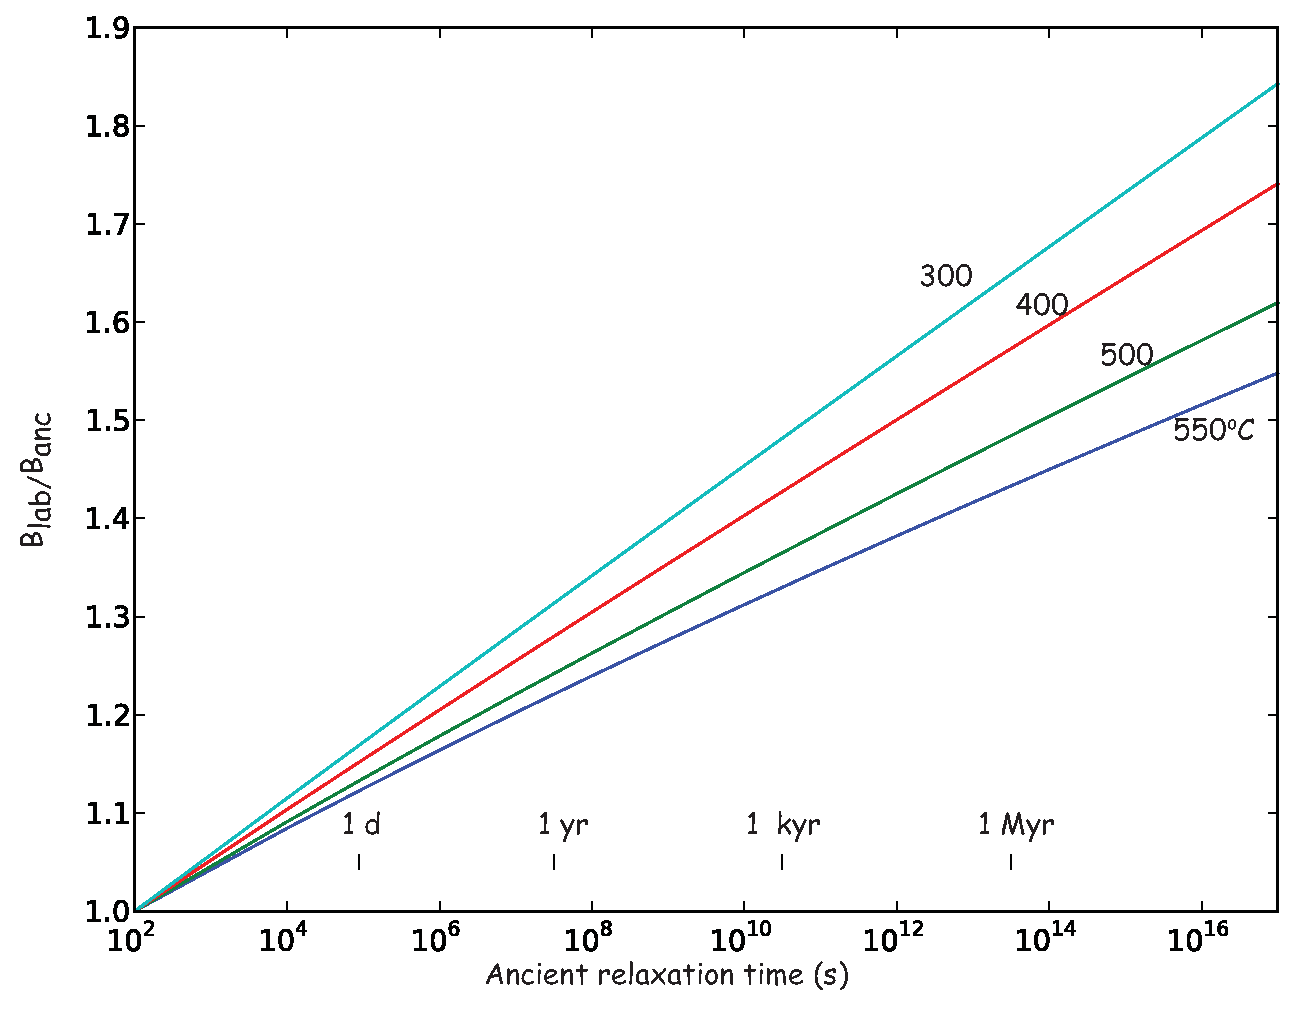
\includegraphics[width= 10 cm]{EPSfiles/coolingrate.eps}
\caption{Ratio of estimated field intensity $B_{est}$ to actual ancient field intensity $B_{anc}$ versus the ratio of cooling rates at the blocking temperature using the method of Halgedahl et al. (1980) but the variation of $M_s(T)$ in Chapter 3 ($\gamma=0.38$).  Laboratory blocking temperatures are shown as examples. [Figure courtesy of R. Mitra.] }
\label{fig:coolingrate}
\end{figure} \nocite{selkin00b}

\subsection{Reducing the effect of heating}

The previous section was devoted to experiments in which detection of non-ideal behavior is done by repeating various temperature steps.   The full IZZI experiment, including TRM acquisition tests and perhaps even TRM anisotropy or non-linear TRM acquisition tests involves many heating steps (as many as 50!).    Each time a specimen is heated, it is exposed to the risk of alteration.   Some experimental designs focus on reducing the number of heating steps or the type of heating to minimize the frequently catastrophic consequences of laboratory heating on the results.   

There are a number of strategies for reducing the effects of laboratory heating.    These include using controlled atmospheres, reduced number of heating steps and reduced heating of the matrix with microwaves focussed on the ferromagnetic components of the specimen.  


\subsubsection{Controlled atomospheres}

Thellier and Thellier (1959) tried heating specimens in neutral atmospheres.  This requires either placing the specimen in a vacuum or a chemically neutral atmosphere.  There are technical difficulties and most researchers have found minimal improvement in their results.   

\subsubsection{Perpendicular field method}

Reducing the number of heating steps has been approached in several ways. 
\index{paleointensity method!perpendicular field}
\index{Kono, M.}
\index{Ueno, N.}
 Kono and Ueno (1977) \nocite{kono77} describe in detail a  single heating step per temperature method  originally  suggested by
 \index{Kono, M.}
  Kono (1974).  \nocite{kono74} Assuming that the specimen has a single component of magnetization, which can be  isolated after demagnetizing  at some low temperature (100$^{\circ}$C),   the specimen is heated in a laboratory field \ applied perpendicular to the NRM.  $M_{ pTRM}$ is gotten by vector subtraction.  The goal is that by reducing the number of heatings,  the alteration can be reduced  to some extent.  This method requires strictly uni-vectorial NRMs (an assumption that is difficult to test with the data generated by this method) and rather delicate positioning of specimens in the furnace or fancy coil systems that generally have a limited region of uniform field, reducing the number of specimens that can be analyzed in a single batch.    Steps like the pTRM checks and pTRM tail checks are possible with this method, but they necessitate additional (zero field) heating steps.   
 
 \subsubsection{Multi-specimen techniques}
 
A second strategy for reducing the number of heating steps is to treat multiple specimens from a single cooling unit as a homogeneous set and expose each specimen to a limited subset of all the heating steps required for a complete paleointensity experiment.   These ``multi-specimen'' techniques derive from one proposed by 
\index{Hoffman, K.A.}
Hoffman  et al. (1989). \nocite{hoffman89}  Recent incarnations include  Hoffman and 
\index{Biggin, A.}
Biggin (2005) and   
\index{Dekkers, M.}
\index{B\"ohnel, H.}
Dekkers and B\"ohnel (2006).  \nocite{hoffman05,dekkers06}  The basic idea is to take multiple  specimens from a given cooling unit and subject them to a reduced number of heating steps.    The data are stacked to yield a single paleofield estimate.  The Hoffman-Biggin (2005) method has some estimate of the effects of alteration by including at least one double heating step.  The method of Dekkers and B\"ohnel (2006) is somewhat different in that pTRMs are imparted at a temperature thought to exceed the overprint unblocking but be less than the onset of chemical alteration.  Each specimen is treated in different laboratory field strength in  a field parallel to the NRM direction.    This technique has been sold as being applicable to multi-domain remanences, but the inequality of blocking and unblocking makes this invalid.   Moreover, there are few ways to check the assumptions of uni-vectorial NRM, lack of alteration in the lab and the insidious effect of pTRM tails.   



\subsubsection{Shaw family of experiments}
\label{sect:shaw}


The previous sections were devoted to experiments in which detection of non-ideal behavior is done by repeating various temperature steps.    In this section we will briefly introduce an alternative approach, long in use in paleointensity studies, the so-called 
\index{paleointensity method!Shaw}
{\it Shaw method}  (e.g., 
\index{Shaw, J.}
Shaw, 1974).  \nocite{shaw74}There are many variants of the Shaw method and the reader is referred to 
\index{Tauxe, L.}
\index{Yamazaki, T.}
Tauxe and Yamazaki (2007)  \nocite{tauxe07} for a recent review.  In its simplest form, we measure the NRM, then progressively demagnetize it with alternating fields (AF) to establish the coercivity spectrum of the specimen prior to heating.  The specimen is then given  an anhysteretic remanence ($M_{ARM_1}$; see Chapter 7).   The use of anhysteretic remanence is usually rationalized by pointing out that   in many ways  it  is analogous to the original TRM (see 
\index{Dunlop, D.J.}
\index{\"Ozdemir, \"O.}
Dunlop and \"Ozdemir, 1997).   $M_{ARM_1}$ is then progressively demagnetized to establish the relationship between the coercivity spectrum of the $M_{NRM}$ (presumed to be a thermal remanence) and $M_{ARM_1}$  prior to any laboratory heating. 
As with the step-wise heating  methods, $M_{NRM}$ is normalized by a laboratory thermal remanence.  But in the case of the Shaw type methods, the specimen is given a total TRM, ($M_{TRM_1}$) which is AF demagnetized as well.  Finally, the specimen is given a second ARM ($M_{ARM_2}$) and AF demagnetized for the last  time.    

\begin{figure}[htb]
%\epsfxsize 14cm
%\centering \epsffile{EPSfiles/Shaw-DD.eps}
\centering  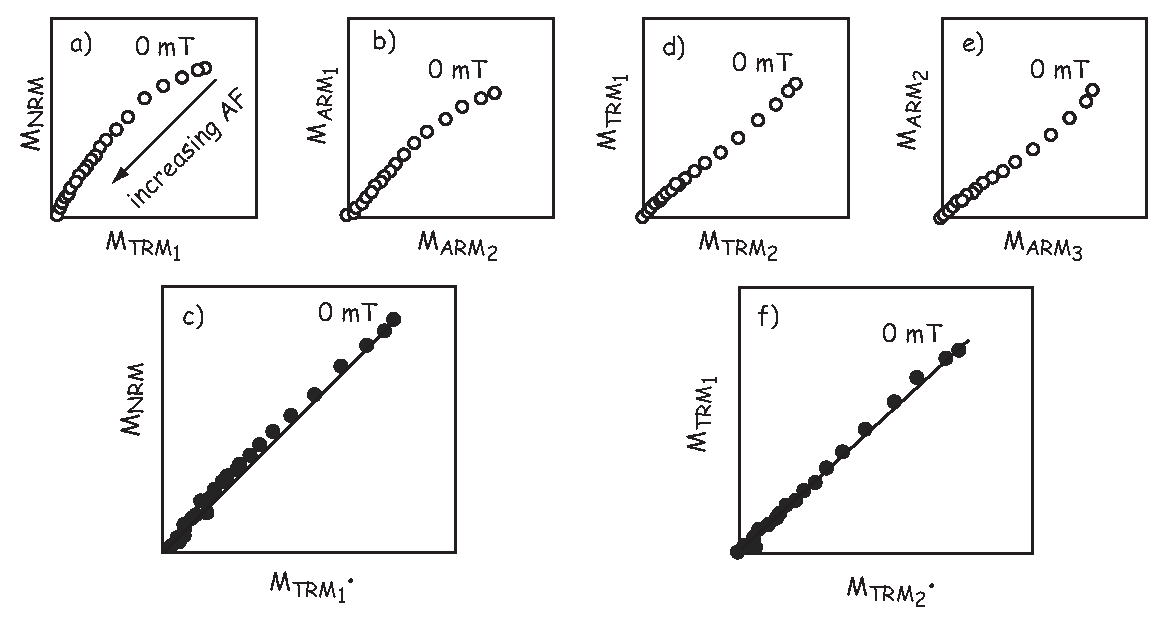
\includegraphics[width=14 cm]{EPSfiles/Shaw-DD.eps}
\caption{ Shaw family of methods (see text).    a) Plot of pairs of NRM and the first TRM for each AF demagnetization step.  b) Plot of pairs of the first ARM and the second ARM for each AF demagnetization step.  c) Plot of pairs of NRM and TRM adjusted by the ratio of ARM1/ARM2 for that AF step from b) (TRM1*).  d) same as a) but for the first and second TRMs.  e) same as a) but for the second and  third ARMs.  f) Same as c) but for first and second TRM where TRM2* is adjusted using ARM2/ARM3 ratio from e). [Data of  Yamamoto et al., 2003; figure from Tauxe and Yamazaki, 2007.]}
\label{fig:shaw-dd}
\end{figure} \nocite{yamamoto03,tauxe07}

The basic experiment is shown in Figures~\ref{fig:shaw-dd}a and b.  If the first and second ARMs do not have the same coercivity spectrum as in Figure~\ref{fig:shaw-dd}b, the coercivity of the specimen has changed and the NRM/TRM ratio is suspect.  

There are many variants of the Shaw method that seek to improve reliability or success rate and the reader is referred to a review by 
\index{Tauxe, L.}
\index{Yamazaki, T.}
Tauxe and Yamazaki (2007) for a more complete discussion.
  The primary reasons stated for using Shaw-type methods as opposed to the theoretically more robust step-wise heating methods  are:  1) they are faster, and 2) because the specimen is only heated once (albeit to a high temperature), alteration may be  minimized.    The first rationale is no longer persuasive because modern thermal ovens have high capacities  and step-wise heating methods are certainly not slower than the Shaw method on a per specimen basis, if one analyzes lots of specimens.  This is particularly true for the more elaborate Shaw family protocols currently in use.      The second rationale may have  some validity and warrants further work.  The key features of any good experiment are the built-in tests of the important assumptions and current designs of Shaw type experiments do not build in the necessary checks. 
  

 
  Several alternative approaches have been proposed which instead of detecting non-ideal behavior such as alteration, attempt to minimize it (see
  \index{Tauxe, L.}
\index{Yamazaki, T.}
 Tauxe and Yamazaki, 2007 for more complete discussion).  These methods include reducing the number of heating steps required (as in the Shaw methods), heating specimens in controlled atmospheres, reducing the time at temperature by for example measuring the specimens at elevated temperature, or using microwaves to excite spin moments as opposed to direct thermal heating.     Of these, the microwave paleointensity approach is perhaps the most popular and we will briefly discuss that here.  

 
\subsubsection{Use of microwaves for thermal excitation}

Until now we have not concerned ourselves with HOW the magnetic moment of a particular grain becomes unblocked.  Earlier, we mentioned ``thermal energy'' and left it at that. But how does thermal energy do the trick?  

   An external magnetic field generates a torque on the electronic spins, and in isolation, a magnetic moment will respond to the torque in a manner similar in some respects to  the way a spinning top responds to gravity: the magnetic moment will precess about the applied field direction, spiraling in  and come to a rest parallel to it. Because of the strong exchange or superexchange coupling  in magnetic phases, spins tend to be aligned parallel (or antiparallel) to one another and the spiraling is done in a coordinated fashion, with neighboring spins as parallel as possible to one another.  This phenomenon is known as a 
   \index{spin waves}
 spin wave  (see Figure~\ref{fig:spinwave} in Chapter 3).  
 
 Raising the temperature of a body transmits energy (via {\it phonons})  to the electronic spins, increasing the amplitude of the spin waves.   This  magnetic energy is quantized in {\it magnons}.    In the traditional step-wise heating experiment, the entire specimen is heated and the spin waves are excited to the point that some spin vectors may flip their moments as described in  Chapter  7. 
 
  
 As in most kitchens, there are two ways of heating things up: the conventional oven and the microwave oven.  In the microwave oven, molecules with certain vibrational frequencies (e.g., water) are excited by 
\index{paleointensity method!microwave}
 microwaves.  These heat up, passing their heat on  to the rest of the pizza (or whatever).  If the right microwave frequency is chosen, ferromagnetic particles can also be excited directly, inviting the possibility of heating only the magnetic phases, leaving the matrix alone (e.g., 
 \index{Walton, D.}
 Walton et al., 1993).  \nocite{walton93} The rationale for developing this method is to reduce the degree of alteration experienced by the specimen  because the matrix often remains relatively cool, while the ferromagnetic particles themselves get hot.  But, the magnons get converted to phonons, thereby transferring the heat from the magnetic particle to the matrix encouraging alteration (even melting sometimes!).  So, while alteration may in fact be reduced (see, e.g., 
 \index{Hill, M.J.}
 Hill et al. 2005), it has not yet been eradicated.  \nocite{hill05}
 
The same issues of non-linearity, alteration,  reciprocity, anisotropy and cooling rate differences, etc.,  arise in the microwave approach as in the thermal approach.  Ideally, the same experimental protocol could be carried out with microwave ovens as with thermal ovens.  In practice, however, it has been quite difficult to repeat the same internal temperature,  making double (or even quadruple) heatings challenging.  Yet tremendous strides have been made recently in achieving reproducible multiple heatings steps (e.g., 
 \index{Hill, M.J.}
 Hill et al., 2005).  \nocite{hill05}

 It is likely that the issues of reciprocity of blocking and unblocking in the original (thermally blocked) and the laboratory (microwave unblocked) and differences in the rate of blocking and unblocking will remain a  problem for some time as they have for thermally blocked remanences.   
It is also worth noting that the
theoretical equivalence between thermal unblocking and microwave unblocking has not yet been demonstrated.    Nonetheless, if alteration can be prevented by this method, and the theoretical underpinnings can be worked out, it is well worth pursuing.
 
\subsubsection{Using materials resistant to alteration}
 
 Another very important approach to the paleointensity problem has been to find and exploit materials that are themselves resistant to alteration.      There are an increasing variety of promising materials, ranging from quenched materials, to single crystals extracted from otherwise alteration prone rocks,  to very slowly cooled plutonic rocks (e.g., layered intrusions).       Quenched materials include volcanic glasses (e.g.,
 \index{Pick, T.}
 \index{Tauxe, L.}
  Pick and Tauxe , 1993; Tauxe 2006),  metallurgical slag (e.g., 
  \index{Ben-Yosef, E.}
  Ben-Yosef et al., 2008) and  welded tuffs (unpublished results).    Single crystals of plagioclase extracted from lava flows (see review by 
  \index{Tarduno, J.A.}
  Tarduno et al., 2006) \nocite{tarduno06} can yield excellent results while the lava flows themselves may be  prone to alteration or other non-ideal  behavior.    Parts of layered intrusions (e.g., 
 \index{Selkin, P.}
 Selkin et al., 2000b) can also perform extremely well during the paleointensity experiment.   \nocite{pick93,tauxe06b,selkin00,tarduno06}    
 

  
\subsubsection{Use of IRM normalization}

  Sometimes it is difficult or impossible to heat specimens because they will alter in the atmosphere of the lab, or the material is too precious to be subjected to heating experiments (e.g., lunar samples and  some archaeological artifacts).   If TRM is linear with the applied field, there may be an alternative for order of magnitude guesstimates for paleointensity without heating at all.  TRM normalized by a saturation remanence ($M_r$) can be  quasi-linearly related to the applied field  up to some value depending on mineralogy and grain size population.    
  
TRM/IRM can   at best only give  an order of magnitude estimate for absolute paleointensity and that only for ideal, equant, and small SD magnetic assemblages (see Chapter 7 for theoretical treatment).  These strict constraints may make even an order of magnitude guess unreliable.  Finally,  multi-domain TRMs and IRMs do not respond similarly under AF demagnetization, the former  being much more stable than the latter.     Nonetheless, if magnetic uniformity can be established, it may in fact be useful for establishing relative paleointensity estimates;  thisis done routinely in sedimentary paleointensity studies as we shall see later in the chapter.  The caveats concerning  single component remanences  are still applicable and perhaps complete AF demagnetization of the NRM would be better than a single ``blanket'' demagnetization step.   Moreover,  we should bear in mind that for larger particles, TRM can be  strongly non-linear with applied field at even relatively low fields (30 $\mu$T) according to the experimental results of
  \index{Dunlop, D.J.}
  \index{Argyle, K.S.}
\nocite{dunlop97b}
Dunlop and Argyle (1997).   The problem with the IRM normalization approach is that domain state, linearity of TRM,  and the  nature of the NRM cannot be assessed.  The results are therefore difficult to interpret in terms of ancient fields.  

\subsection{Quality assurance and data selection}

Given the number of key assumptions in the paleointensity method and the growing complexity of the modern experimental design, there are a bewildering array of statistics that can be calculated to assess the quality of a given data set.    Many of these are defined in Appendix~\ref{app:pint} to which the reader is referred for a detailed explanation.    There is at present no consensus on which statistics guarantee the reliability of a given result.    It is safe to say that the more tests performed (and passed), the greater the confidence in the results.  And, the more replicate specimens  that are measured and the more samples from different recording media,  that are measured yielding consistent results, the more confidence we can have in the conclusions.  This is a rapidly developing area of research, so stay tuned!





\section{Paleointensity with DRMs}
\label{sect:drmint}

\index{paleointensity method!relative}
The principle on which paleointensity studies in sedimentary rocks rests is
that DRM is linearly related to the magnitude of the
applied field $\B$.   We learned in Chapter 7  that this is  unlikely to be universally true, yet it is the foundation  of all relative paleointensity studies published to date.  
Forgetting for the moment that non-linear behavior may in fact be frequently found in nature, we will proceed with a discussion of paleointensity in sediments making the first order assumption of linearity.  

\begin{figure}[htb]
%\epsfxsize 10cm
%\centering \epsffile{EPSfiles/drm1.eps}
\centering  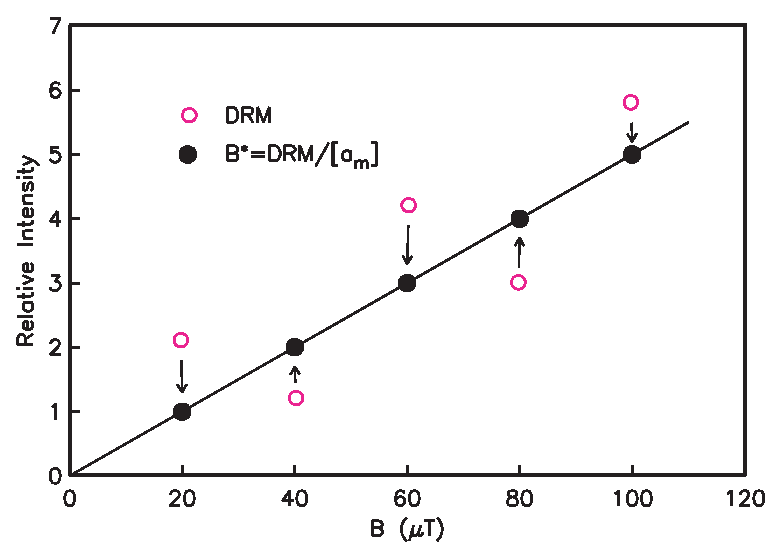
\includegraphics[width=10 cm]{EPSfiles/drm1.eps}
\caption{Principles of relative paleointensity.  The original DRM is plotted
as open symbols.  It is a function not only of the applied field, but
also of the magnetic activity $[a_m]$ of the specimen.  When normalized by
$[a_m]$ (dots), the DRM is a linear function of applied field $B$.  [Redrawn from Tauxe, 1993.] }
\label{fig:drm}
\end{figure}
\nocite{tauxe93}



Following from the introductory discussion of paleointensity in general, we would require a laboratory redeposition experiment that duplicates the natural remanence acquisition process in order to be able to determine absolute paleointensity in  sediments.  
The problem with sedimentary paleointensity data is that laboratory
conditions can rarely (if ever) achieve this.  Assuming that the remanence is not chemical but depositional in origin,
  the intensity of remanence is still a complicated  function
  of applied  field, magnetic mineralogy, concentration,  and even chemistry of the water column.

Under the ideal conditions depicted in Figure~\ref{fig:drm}, the initial
DRM of a set of specimens deposited under a range of magnetic field
intensities ($B$) is shown as open circles.  The
relationship is not linear because each specimen has a different 
response   to the applied field (here called 
\index{magnetic!activity}
magnetic activity $[a_m]$) as a result of differences in
the amount of magnetic material, magnetic mineralogy, etc.
For example, specimens with a higher concentration of magnetic
material will have a higher DRM.  If $[a_m]$ can be successfully
approximated, for example, by bulk remanences such as IRM or ARM,
or by $\chi_b$ (Chapters  7 and Chapter 8), then a
normalized DRM (shown as dots in Figure~\ref{fig:drm}) will reflect at least  the
relative intensity of the applied field. 


Our theoretical understanding of DRM is much less developed than for TRM
(Chapter  7).  Because of the  lack of a firm theoretical foundation for
DRM, there is no simple method for determining  the appropriate normalization parameter.  In Chapters  7  and 8 we considered a variety of theoretical aspects of DRM and various parameters potentially useful for normalization.  Many proxies
have been proposed  ranging from normalization by bulk magnetic properties such as ARM, IRM, or  $\chi_b$ or more complicated proxies involving selective demagnetization of the NRM or normalizer or both.    One can imagine that even more sophisticated normalization techniques could be devised by targeting particular coercivity fractions discovered by the IRM component diagrams discussed in Chapter 8.  

\index{Tauxe, L.}
Tauxe et al. (2006) \nocite{tauxe06} summarized two major complications in our quest for meaningful relative paleointensity estimates from sediments.  First, the size of the floc in which magnetic moments are embedded plays a huge role in the DRM strength, yet estimating original floc size in sediments is a daunting task.  Second, DRM is only approximately linearly related to the applied field for the larger floc sizes;  small flocs or isolated magnetic particles are likely to be highly non-linear in their magnetic response.  

How can sedimentary relative paleointensity data be judged?  Here  are some thoughts:


\begin{enumerate}
\item The natural remanence must be carried by a detrital phase of high magnetic stability.
 Furthermore, the portion of the natural remanent
vector used for paleointensity should be  a single, well defined component of
magnetization.   The nature of the NRM can be checked with progressive demagnetization using AF and thermal techniques.  Supplementary information from hysteresis and rock magnetic experiments can also be useful. 

\item  The detrital remanence must be an excellent recorder of the geomagnetic field, exhibit no inclination error and if both polarities are present the two populations should be antipodal.   The associated directional data must therefore be plotted on equal area projections whenever they are available.   

\item Large changes in concentration (more than about an order of magnitude) and any change in    magnetic mineralogy  or  grain size will foil attempts at normalization.   These changes can be detected with the use of bi-plots of, for example, IRM and $\chi$ (see Chapter 8).  Such bi-plots should be linear, with low scatter.


\item The relative paleointensity estimates that are coherent with bulk rock
magnetic parameters should be treated with caution.  Coherence can be assessed using standard spectral techniques.  

\item  Records from a given region should be coherent within the limits of a common time
scale.   Whenever possible duplicate records should be obtained and compared. 

\item For a relative paleointensity record to have the maximum utility, it should have an independent time scale.  Many deep sea sediment records are calibrated using oxygen isotopic curves or magnetostratigraphic age constraints (or both).  Lake sediments are more difficult to date and rely for the most part on radiocarbon ages.  

\item Changes in water chemistry (pH and salinity) and changes in clay mineralogy or concentration can have a huge effect on the tendency to flocculate.  Such changes are likely to have a profound effect on the DRM, yet may be difficult to detect after the fact.  Low salinity environments (lakes) are particularly sensitive to this problem.    In any case, all studies should probably attempt to characterize changes in the clay fraction, yet very few (if any) have done so to date.  
\end{enumerate}

\noindent SUPPLEMENTAL READINGS: Dunlop and \"Ozdemir (1997), Chapters 8 and 15; \nocite{dunlop97}
Valet (1998); \nocite{valet98}
Tauxe and Yamazaki (2007). \nocite{tauxe07}


\section{Problems}

{{\parindent 0pt  \parskip 12pt

{\bf Problem 1 }

a)  In this problem, we will use published data to get a feel for ``real'' paleointensity data.  Make sure you have the {\bf PmagPy} programs working (see \href{http://earthref.org/PmagPy/cookbook/}{PmagPy webiste}).  You can find a data set associated with a particular publication (if someone uploaded the data), by using the digital object identifier (DOI) search.  For example, the data set of Shaar et al. (2011)  \nocite{shaar11} could be located using the syntax:   

\url{http://earthref.org/doi/10.1016/j.epsl.2010.11.013} 	
	
When you locate the reference, click on the text file icon under the column labeled ``Data''.     This is a dataset   from  Israeli/Jordanian metallurgical slags.   

b) Create a new folder for these data and put the downloaded text file in it.  Make sure it is a directory with no spaces in the path name.

c) Open a \href{http://earthref.org/PmagPy/cookbook/#command_line}{terminal window} (command prompt on Windows machines).    On the command line,  type:  {\bf QuickMagIC.py}. Change directories into your ``Project Directory''. 

d) Click on the  ``unpack downloaded txt file'' button on the front panel and choose the file you downloaded. 

e) Click on the `Thellier GUI' button.  

f) Step through the data by clicking on `next'.  You don't have to look at all of them, because there are a LOT.  

g)  You will be able to see the interpretations used in the publication.  Perhaps you would interpret the data differently.  To change an interpretation, change the  temperature bounds for the slope calculation.  A complete list of the definitions for paleointensity statistics used by the GUI is available as a supplement to the article by \href{#http://dx.doi.org/10.1002/2013GC005135}{Paterson et al., 2014}  \nocite{paterson14} and available for download   \href{http://onlinelibrary.wiley.com/store/10.1002/2013GC005135/asset/supinfo/ggge20412-sup-0001-suppinfoCORRECTED.pdfv=1&s=e1c3ab0a86c942d1039f6d2e15496aa172dc86ec}
{here}.
 
  
 You can see how the answer will  change with different boundary picks and also whether the interpretation `passes' or not.  
 
h)     The selection criteria can be changed by choosing  Analysis $=> $Acceptance criteria =$>$change acceptance criteria.   After changing these,  you can try to run the auto interpreter to see what will `pass'.  


i) What do you think were the guiding principles that the original author used to select bounds?  Do you think these are reasonable?  What principles would YOU use to guide your interpretations of these data?   Which statistics are the most useful?  


{\bf Problem 2}

a) Now go to permalink: 

\url{http://earthref.org/MagIC/doi/10.1111/j.1365-246X.1997.tb04082.x} 

and download the data as before.  Make a new project directory and copy the downloaded file into it.       Unpack the txt file with {\bf QuickMagIC.py}.   


b) Find your \href{http://earthref.org/PmagPy/cookbook/#command_line}{command line} and change directories into your new project directory by typing {\it cd MY\_DIRECTORY}, where you type the directory name instead of MY\_DIRECTORY. Then type  {\bf biplot\_magic.py}.    This will give you a list of available options for plotting measurement data.   In this case they are 'LT-AF-Z', 'LT-AF-I', 'LT-IRM', 'LP-X', which are `method codes' in MagIC.   On the \url{http://earthref.org/MAGIC}  website, follow the link to ``Method Codes''.   Examine the available options under  ``Lab Protocol'' and ``Lab Treatment''  and find the option that describes   these.   

c) Type:  {\bf biplot\_magic.py}.   Using the help message for this program (remember the -h option), figure out how to plot ARM versus $\chi$ and IRM versus $\chi$ for these data.    

d) Use the program {\bf strip\_magic.py} to plot relative intensity versus age.     

e)  These data are supposedly relative paleointensity data from the Oligocene in the South Atlantic.  What would convince you that these were ``real''?   


}






